\documentclass[12pt]{article}
\usepackage[T1]{fontenc}
\usepackage[margin=1in]{geometry}
\usepackage{amsmath,amssymb}
\usepackage{graphicx}
% A clone receives no PNG under paper/ (the .gitignore paper/** rule), so the
% bare \includegraphics names below resolve only for someone who already holds
% the untracked copies. These are the tracked originals: figures/ carries the
% twelve generated figures, and the Monte Carlo panel belongs to the fold-in
% production run (abm/monte_carlo_trapped_liquidity.png is the Berger run and is
% NOT the panel this manuscript prints).
\graphicspath{{./}{../../figures/}{../../abm/data/runs/run-2026-07-04-15yr-foldin/}}
\usepackage{float}
\usepackage{array}
\usepackage{longtable}
\usepackage{booktabs}
\usepackage{threeparttable}
\usepackage{caption}
\usepackage{authblk}
\usepackage[authoryear,round]{natbib}
\usepackage{xurl}
\usepackage[hidelinks]{hyperref}
\usepackage{microtype}
\usepackage{setspace}
\emergencystretch=1.5em
\renewcommand{\thesection}{\Roman{section}}
\renewcommand{\thesubsection}{\thesection.\Alph{subsection}}
% Possessive citation: one macro so a bibliography change cannot desynchronize
% hand-rolled \citeauthor{X}'s (\citeyear{X}) constructions.
\newcommand{\citepos}[1]{\citeauthor{#1}'s (\citeyear{#1})}

\title{Mortgage Lock-In and Federal Reserve MBS Runoff: A Model-Based Decomposition}
\author{Eugene Ong}
\affil{Carnegie Mellon University}
\date{October 10, 2026}
\begin{document}
\maketitle
\begin{abstract}
\noindent From June 2022 through November 2025, Agency-MBS caps exceeded the net decline in holdings by \$764.7 billion. The cap is not a no-lock-in counterfactual: allocating the New York Fed's May 2022 projection gives an expectations-relative gap of \$87.8--\$186.8 billion. I combine SOMA holdings, Freddie Mac composition, an imported moving response, and a turnover floor in paired response-on and response-off simulations. At the hard-maximum specification, assumed moving shares of $0/25/50/100\%$ yield $0/+1.8/+3.4/+5.6$ points of the cap gap. The \$42.6 billion full-share result is not an empirically preferred estimate. At the same 4.991\% annual floor, a 75--150 PSA sweep spans $+0.9$ to $+15.6$ points; the survival-combination form gives $+11.2$ at 100 PSA. Scaling the opening book once reduces the marginal to \$37.0 billion. Agency-vintage coverage is 51.0\% (July 2026); joint-cell support is 47.6\% (June 2022). Whole-pool-scaled dollars do not measure either slice's contribution. On legacy inputs, response-on predictions overstate voluntary prepaid principal by 23\%; a development candidate still underperforms the cohort-speed baseline. The moving share is unestimated, portfolio transport is incomplete, and these conditional comparisons are neither a common confidence interval nor a newly identified causal effect. The aggregate calibration inputs remain subject to a full source-data audit.
\end{abstract}
\vspace{0.5\baselineskip}
{\footnotesize\noindent\textbf{Keywords:} mortgage prepayment; lock-in; quantitative tightening; agency MBS; conditional simulation.\\
\textbf{JEL codes:} E52, E58, G21, R31.\par}
\newpage
\doublespacing
% Current economics-review revision. Prior source is preserved in reviewed_archive/.
\section{Introduction}\label{sec:intro}

From June 2022 through November 2025, the announced Federal Reserve agency mortgage-backed securities (MBS) runoff caps exceeded the net decline in SOMA current face by \$764.7 billion. That difference is an accounting gap, not the effect of mortgage lock-in. A cap specifies how much principal may run off; it does not guarantee that mortgages will generate that principal. Unlike Treasury maturities, mortgage cash flows depend on amortization, refinancing, home sales, and the surviving distribution of borrower coupons.

Mortgage lock-in can slow those cash flows. A homeowner with a fixed mortgage rate below the current market rate generally gives up valuable financing when selling and purchasing another home. Empirical studies document lower mobility and loan termination at larger mortgage-rate gaps \citep{berger2021,eichenbaum2022,liebersohn2024,batzer2024,fonseca2024}. Mortgage-pricing research models the resulting prepayment and duration risk through borrower heterogeneity, seasoning, burnout, and competing default \citep{dunn1981,richard1989,schwartz1989,stanton1995,deng2000}. This paper connects that household evidence to the accounting of Federal Reserve MBS runoff.

The first contribution is to separate three objects. The cap-relative gap compares an operational ceiling with realized net holdings decline. An expectations-relative gap compares the New York Fed's published May 2022 holdings projection with that decline. A model marginal compares two simulated cash-flow paths, with an imported moving response switched on and off. They answer different questions and cannot be added. Under uniform within-year allocation, the projection-relative gap is \$87.8 billion; a settlement-aware allocation gives \$186.8 billion. Thus the published projection anticipated 75.6--88.5\% of the cap-relative gap under these two constructions, although it may already incorporate lock-in and conditions on a different interest-rate path.

The second contribution is a reproducible, assumption-sensitive portfolio translation. The paper does not claim to identify a new causal elasticity. Freddie Mac loans supply the borrower distribution; an external estimate supplies the response to the rate gap; a baseline prepayment schedule, turnover floor, and reporting convention turn hazards into dollars. Applying the imported response to assumed shares of $0/25/50/100\%$ of voluntary prepayment yields $0/+1.8/+3.4/+5.6$ percentage points of the cap gap. The final case is \$42.6 billion, a named specification rather than an empirically preferred estimate. The sale-related share is unestimated because the available payoff flag does not distinguish sales from refinancing.

Other assumptions are equally consequential. At the 4.991\% annual turnover floor and full moving share, changing the baseline from 75 to 150 PSA moves the marginal from $+0.9$ to $+15.6$ points. Combining baseline and responsive turnover on the survival scale gives $+11.2$ points at 100 PSA. Scaling the opening portfolio once, rather than rescaling reported flows to observed holdings each month, reduces the saved-sample marginal from \$42.6 to \$37.0 billion. These are separate scenario comparisons, not a joint confidence interval or bounds over all mortgage models.

The evidence does not support calling the calculation independently validated. In a frozen retrospective check on January 2024--September 2025 cohort outcomes, response-on predictions overstate voluntary prepaid principal by 23.2\% and have greater exposure-weighted error than a simple 2023 cohort-speed baseline. The response improves on the response-off model, but not on that comparator. The paper therefore treats its simulated dollars as conditional accounting results. Its policy implication is correspondingly specific: regularly publish cap and projected cash-flow paths together, separating interest-rate and prepayment-assumption scenarios.

\section{Institution, Data, and Benchmarks}\label{sec:data}

\subsection{Runoff policy and net holdings}

The monthly agency-MBS cap was \$17.5 billion during June--August 2022 and \$35 billion from September 2022. The 2024 and 2025 runoff slowdowns reduced Treasury caps, not the MBS cap. Reinvestment did occur during the phase-in: the New York Fed reports \$32.8 billion of MBS purchases in the June, July, and August purchase periods. It reports no purchases from the September purchase period through the end of 2022 because principal payments were below the cap \citep[p.~15]{nyfedomo2022}. Purchase periods and settlement dates differ, so those transactions cannot be assigned mechanically to calendar-month holdings changes. The September Teller Window explanation describes the operating mechanics; it is not the source of the May projection \citep{nyfed2022}.

Let $C_t$ denote the announced cap and $H_t$ SOMA current face. The named cap-relative accounting object is
\begin{equation}
G_C=\sum_{t=\mathrm{Jun22}}^{\mathrm{Nov25}}\{C_t-(H_{t-1}-H_t)\}
=1{,}417.5-652.7517468=764.7482532
\quad\text{(\$ billions)}.
\label{eq:benchmark}
\end{equation}
The displayed benchmark is \$764.748 billion. It measures caps less net face decline, not caps less gross borrower principal receipts. Principal payments reduce face; settlements of earlier purchases and reinvestments add face. Other reporting adjustments can also affect measured changes. The public SOMA series do not separately report monthly gross principal receipts, reinvestment settlements, and other changes in face. A per-CUSIP reconstruction reproduces the holdings change rather than independently identifying gross remittances.

Figure~\ref{fig:benchmark} shows the original construction. Four inferred monthly prepayment rates are clipped at zero when measured rolloff falls below scheduled amortization. That is a limitation of the holdings-based back-out, not evidence of zero borrower prepayment. Convolving the cap schedule with settlement lags measures sensitivity at the window edges; it does not recover the missing gross-principal series. Appendix~\ref{app:benchmark} records these distinctions and alternative allocations.

\begin{figure}[H]
\centering
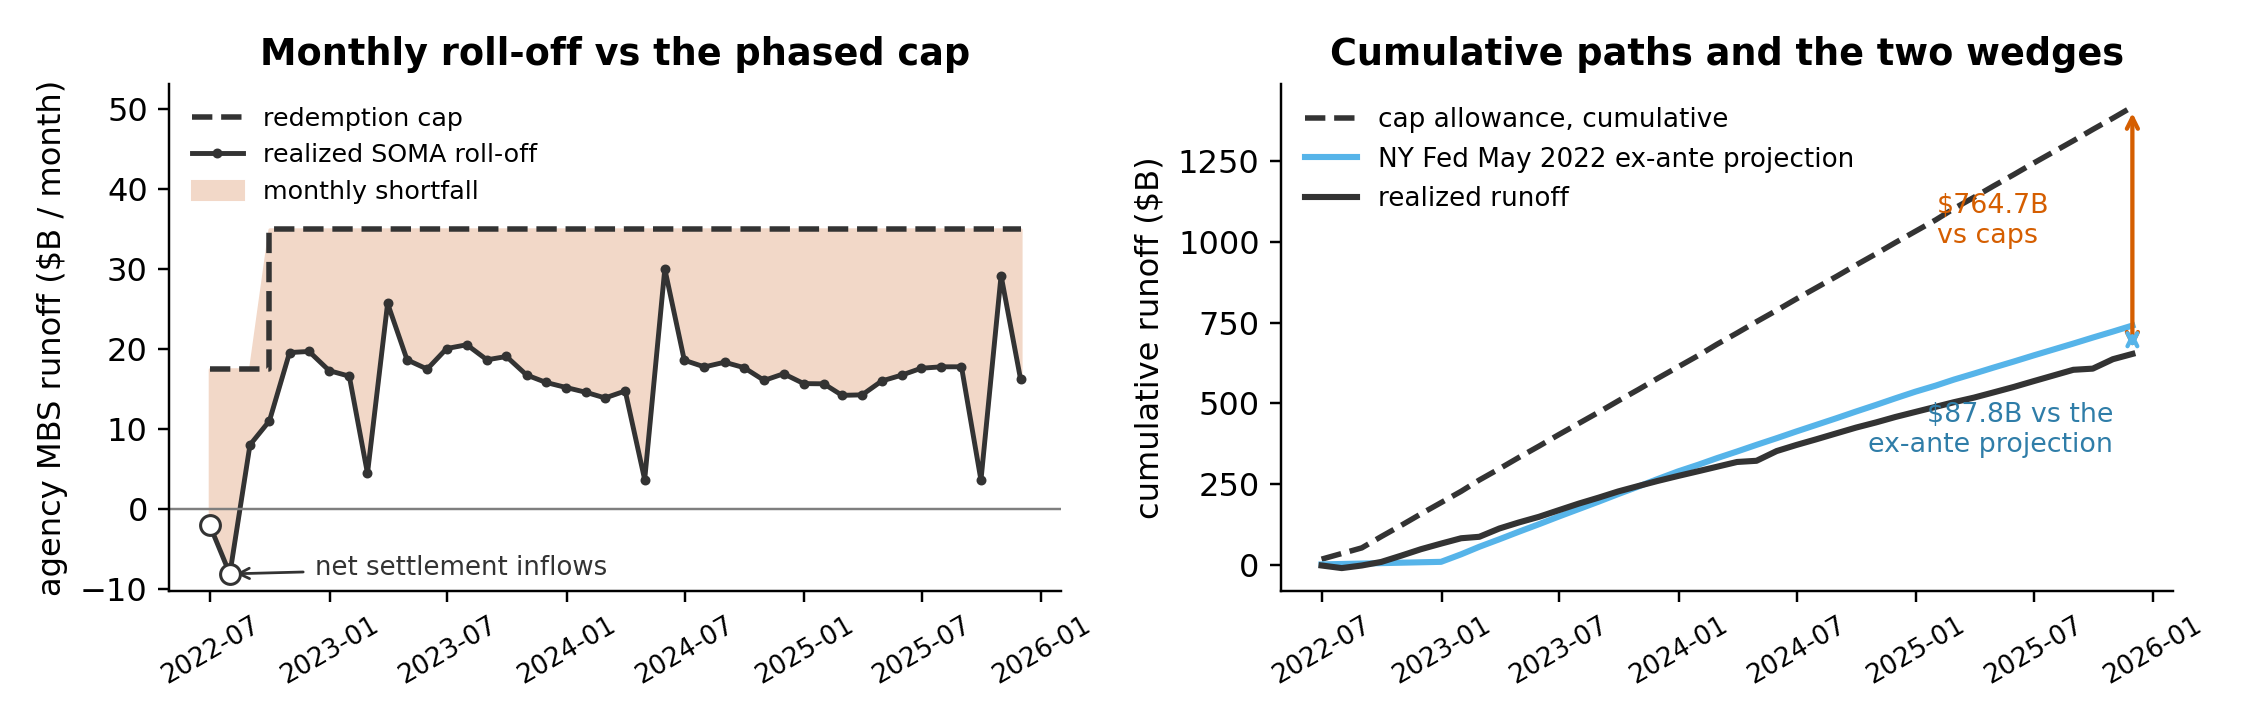
\includegraphics[width=0.94\textwidth]{fig9_benchmark_construction}
\caption{Caps, realized net face decline, and the published projection. The terminal cap-relative gap is \$764.748 billion. The displayed projection uses uniform within-year allocation and gives an \$87.8 billion gap. Net holdings changes include settlement effects; neither the monthly back-out nor the cap path is a measure of gross principal receipts.}
\label{fig:benchmark}
\end{figure}

\subsection{The expectations-relative benchmark}

The source is \emph{Open Market Operations During 2021}, published in May 2022, Chart 34 on printed page 49 (PDF page 51), with its chart-data workbook, sheet ``Chart 34,'' column D, ``Agency MBS'' \citep{nyfedomo2021,nyfedomo2021data}. The year-end levels for 2021--2025 are \$2{,}615.5, \$2{,}599.6, \$2{,}319.9, \$2{,}072.8, and \$1{,}849.7 billion. The revision retrieves that workbook and matches all five levels exactly. The report cover dates the publication May 2022; the workbook cover's ``May 2021'' text is inconsistent with it. Annual changes must be allocated within years to obtain the study window.

\begin{table}[H]
\centering\small
\caption{Expectations-relative shortfall under two explicit allocations (\$ billions). Anticipated share is $(\sum C_t-\text{projected decline})/G_C$. Neither construction identifies a no-lock-in path.}
\label{tab:benchmarks}
\begin{tabular}{@{}lrrrr@{}}\toprule
Allocation & Projected & Realized & Gap & Anticipated share\\\midrule
Uniform annual net decline & 740.583 & 652.752 & 87.832 & 88.5\%\\
Settlement-aware proxy & 839.530 & 652.752 & 186.778 & 75.6\%\\\bottomrule
\end{tabular}
\end{table}

Uniform allocation spreads each annual net decline across its twelve months and clips the result to June 2022--November 2025. The settlement-aware case assigns a \$92.322 billion proxy for early-2022 inflows outside the QT window, then distributes the adjusted 2022 decline across June--December. It uses realized early-year holdings changes as a proxy, so it is partly retrospective rather than a wholly ex-ante forecast. The two allocations imply the same realized decline but different expectations-relative gaps. Extreme allocations are stress cases in Appendix~\ref{app:benchmark}, not a probability distribution. The projection also uses the spring-2022 expected rate path, which differs from realized rates. Consequently, dividing the model marginal by \$87.8 billion does not estimate the causal share of an unexpected shortfall.

\subsection{Loan data and SOMA coverage}

The saved production sample contains 75,000 Freddie Mac loans originated in 2017--2021, drawn across vintage, coupon, and credit strata. It includes loans whose latest pre-QT observation was already terminated. Simulations use positive active balances. The input histories provide note rates, principal, age, credit, leverage, and delinquency states. A fresh sensitivity sample separately draws 75,000 unique positive-balance, 30-year May-2022 survivors from 6,261,485 eligible loans across all twenty origination quarters. Its seed is 42; its sample, code, and twenty snapshot hashes are verified without repeating raw downloads.

The population restrictions matter for dollars. Conventional 2017--2021 collateral represents 51.0\% of the book in the agency-by-vintage coverage calculation. A different, June 29, 2022 grid contains twelve listed UMBS 30-year coupon-by-vintage cells representing 47.5876\% of total SOMA face. The latter grid omits cells below 0.1\% of face and does not identify the Freddie/Fannie mix. Neither share is a probability-sampling coverage rate. The production sample, saved joint-cell reweight, and fresh survivor reweight are distinct specifications.

\begin{table}[H]
\centering\small
\caption{Population coverage and the role of separate checks. Overlapping exclusions cannot be added.}
\label{tab:coverage}
\begin{tabular}{@{}>{\raggedright\arraybackslash}p{3.9cm}>{\raggedright\arraybackslash}p{2cm}>{\raggedright\arraybackslash}p{7.7cm}@{}}\toprule
Population or check & Book share & Interpretation\\\midrule
Conventional 2017--2021 & 51.0\% & Agency-by-vintage scope; no known SOMA loan inclusion probabilities.\\
Listed UMBS 30-year cells & 47.6\% & Twelve June-2022 cells under the 80 bp bridge; both joint-cell runs expand this pool to total holdings.\\
Ginnie Mae & 20.4\% & External speed overlay; no directly estimated Ginnie hazard or measured assumption take-up.\\
Pre-2017 and 2022 vintages & 10.6\%, 23.1\% & Observed-speed and vintage extensions with proxy assumptions.\\
Fifteen-year MBS & About 9\% & Scheduled-principal/term extension; no separately estimated behavioral hazard.\\
Fannie replication & Separate sample & Conventional-agency transfer check using the same imported response.\\\bottomrule
\end{tabular}
\end{table}

Joint-cell weights match initial balance shares, not later exposures. The assumed note-to-pass-through bridge assigns loans to cells while their actual note rates remain in the hazard. Section~\ref{sec:results} reports 60/80/100 bp perturbations with the same IDs and targets. The fresh versus saved comparison changes both sampling frame and draw and cannot isolate sampling noise. Ginnie, vintage, and term checks address different omissions; none supplies the missing full-SOMA probability sample.

\section{Model and Assumptions}\label{sec:model}

\subsection{Loan-level prepayment model}

Define the positive lock-in gap $g_{it}=100(r_t-c_i)$ in percentage points, with market and note rates $r_t,c_i$ in decimals. Let $P=0.06$ be the reference quarterly moving probability and $d=0.065$ the assumed proportional quarterly reduction per 100 basis points, with a source band of 5.5--7.7\% \citep{liebersohn2024}. The discrete conversion is
\begin{equation}
q(P)=1-(1-P)^{1/3},\qquad
b=\log\!\left\{\frac{q(P(1-d))}{q(P)}\right\}=-0.0685705,
\qquad \beta=-b.
\label{eq:beta1}
\end{equation}
Thus $\beta=0.0686$ and $\exp(-\beta\times3.8)=0.771$ at a 380-basis-point gap. The code stores the negative refinance-incentive gap $c_i-r_t$ and negative coefficient $b$; its exponent $(-b)100(c_i-r_t)$ equals $-\beta g_{it}$. Switching off the response sets $b=0$, retaining the realized rates and every other model input.

The baseline is the PSA seasoning schedule, not the minimum turnover floor. At speed $s$ and age $a$ months,
\begin{equation}
\mathrm{CPR}_0(a;s)=0.06(s/100)\frac{\min(a,30)}{30},\qquad
h_0(a;s)=1-[1-\mathrm{CPR}_0(a;s)]^{1/12}.
\label{eq:psa}
\end{equation}
The named production specification uses 100 PSA, a 6\% annual plateau before borrower covariates. Its rate-responsive monthly voluntary hazard is
\begin{equation}
h^R_{it}=h_0(a_{it};s)\exp\{-\beta g_{it}-0.15z^{\mathrm{FICO}}_i
+0.10z^{\mathrm{LTV}}_i-0.50B_{k(i),t}\}.
\label{eq:pathB}
\end{equation}
Credit and leverage are standardized over the sample. $B_{k(i),t}$ is accumulated prepaid principal divided by original balance in the loan's vintage-coupon-credit stratum, capped at one. These covariate coefficients are calibrated priors, not estimates of the causal runoff response. Appendix~\ref{app:model} gives the default hazard and state ordering.

\subsection{Baseline-turnover specifications}

For annual turnover floor $f_A$, define $f_m=1-(1-f_A)^{1/12}$. All combinations below are monthly probabilities. Let $h^0$ denote equation~\eqref{eq:pathB} with $b=0$. The assumed moving-share mixture is $h^\mu=(1-\mu)h^0+\mu h^R$, before applying the floor. The alternatives are
\begin{align}
h^{\max}_{it}&=\max\{f_m,h^\mu_{it}\},\label{eq:maxfloor}\\
h^{\mathrm{add}}_{it}&=1-(1-f_m)(1-h^\mu_{it}).\label{eq:addfloor}
\end{align}
The latter is a survival combination. The sum $f_m+h^\mu$ is only its small-probability approximation and is not the implemented formula. The maximum censors the response wherever the floor binds. The survival form allows both components but requires a stronger interpretation of them as distinct causes. Neither is selected by causal evidence in this study.

The 4.991\% annual floor is transported from 2018 discount cohorts, with alternative floor readings of 4.70--5.33\%. It describes total observed deep-discount turnover, including potentially voluntary behavior; it is not a measured strictly involuntary hazard or a lock-in-free control group. Housing inventory and financing incentives remain unseparated. At the saved-sample anchor the floor binds in 35.8\% of evaluated response-off loan-months and 68.8\% on the response-on leg. Moving-share $\mu$ is likewise unestimated: the available code-01 voluntary-payoff flag includes prepaid or matured loans without a sale/refinance split. Zero share gives zero marginal by definition; 25\% is not an empirical lower bound.

\subsection{Calibration and simulation}

Each month broadcasts stratum burnout and calculates the rate gap. The model computes prepayment and default probabilities and proportionally normalizes them if their sum exceeds one. In fractional mode, voluntary principal drains each active balance by its prepayment probability. A separate random default trigger changes loan states, and the fractional prepaid amounts update stratum burnout. The Markov matrix then advances delinquent loans. Scheduled amortization is applied to the remaining active balances, and their age advances. Fractional prepayment reduces balances without removing whole borrowers; a partially prepaid loan can also enter delinquency.

Paired legs use the same starting loans, seed 42, rate path, coefficients, and transition rules. Because balances and states evolve, the same rules do not imply identical scheduled-principal dollars. The coefficient's 380-basis-point application extrapolates beyond a local estimate; halving the response slope beyond 200 basis points lowers the off-window marginal to about $+5.1$ points. An extreme transition-matrix comparison moves trapped principal by approximately \$0.39 billion. These are disclosed sensitivities, not independent validation of the imported response.

\subsection{Accounting convention and comparison}

The engine evolves its loan balances and scales them once at initialization. It then separately scales each month's reported voluntary-plus-scheduled principal $P^j_t$ by observed holdings $H_t^{obs}$ divided by END-of-step active pool exposure $E^j_t$:
\begin{equation}
\widetilde P^j_t=P^j_t\frac{H_t^{obs}}{E^j_t},\qquad
\Delta^{obs}=\sum_t(\widetilde P^{off}_t-\widetilde P^{on}_t).
\label{eq:reporting}
\end{equation}
Numerator flows have already occurred when the denominator is measured. This is a monthly flow-reporting convention; it does not reset every loan's balance or define a self-financing observed portfolio. The historical shared accounting layer adds the same externally imposed dollar adjustments to both paths, shifting their levels but leaving their difference unchanged. Cancellation applies only to equal dollar adjustments. Balance-dependent scheduled flows must be recomputed separately on each leg.

The new comparison retains the same underlying loan walks and reports their unrescaled cash principal after the opening scale. It is a closed opening book: no unsettled purchases or later reinvestment mortgages are added. Default transfers remain separate inactive principal claims because the engine supplies no default-recovery cash; curtailment and additions are zero in this comparison. Each month's active and total-principal identities reconcile. This scope cannot be compared in levels with full-book observed net holdings as though both included the same purchases and recoveries.

Mortgage principal also differs from cap-allowed runoff. For each path, allowable runoff is $\min(P_t,C_t)$ and excess $\max(P_t-C_t,0)$ requires reinvestment. The comparison reports both, without inventing reinvestment-pool cash flows. Its marginal measures principal retained by the imported response under a specified reporting convention, not necessarily a change in the Federal Reserve's complete future holdings path.

\section{Results and Retrospective Validation}\label{sec:results}

\subsection{Assumption comparisons}

Table~\ref{tab:mainresults} places the unestimated moving share, PSA baseline, and turnover form together. The hard-maximum anchor is $+5.5716$ points (\$42.6084 billion), at 100 PSA, the 4.991\% floor, full moving share, and the saved sample. The benchmark denominator is equation~\eqref{eq:benchmark}; it is never replaced by the smaller expectations-relative gap. The historical shared-basis levels are 85.7\% response off and 91.3\% response on. Those level fits are calibrated and do not validate the marginal.

\begin{table}[H]
\centering\small
\caption{Hard-maximum anchor and separate assumption comparisons. Unless varied: saved sample, 4.991\% annual floor, 100 PSA, full moving share, maximum form, observed-holdings flow reporting. Points use the exact cap gap; no row is a confidence interval.}
\label{tab:mainresults}
\begin{tabular}{@{}p{8cm}rr@{}}\toprule
Assumption & Marginal (points) & Marginal (\$B)\\\midrule
Moving share 0 (definitional) & 0.0000 & 0.0000\\
Moving share 25\% & 1.8212 & 13.9274\\
Moving share 50\% & 3.3615 & 25.7071\\
Moving share 100\% & 5.5716 & 42.6084\\
\addlinespace\\
75 PSA & 0.8560 & 6.5465\\
100 PSA & 5.5716 & 42.6084\\
125 PSA & 11.4191 & 87.3271\\
150 PSA & 15.6265 & 119.5033\\
\addlinespace\\
Survival-combination form & 11.2070 & 85.7055\\
\bottomrule
\end{tabular}
\end{table}


The 75/100/125/150-PSA comparison gives $+0.8560/+5.5716/+11.4191/+15.6265$ points. It was already present in the saved research artifacts and is promoted here because it materially exceeds the narrow loan-sampling interval. A larger baseline places more loans above the hard floor, where the response can affect principal. PSA and the floor are different assumptions even when their annual numbers are close. The response-off path changes with PSA as well; each row uses its matching pair.

At 100 PSA the survival-combination alternative produces $+11.2070$ points (\$85.7055 billion). Varying the floor and elasticity within the historical joint calibration grid gives $+2.1$ to $+13.2$ points under its specified form. These comparisons are not combined into a synthetic statistical band. An assumed positive response generally produces a positive model marginal; that sign is not new portfolio evidence identifying the response.

\begin{figure}[H]
\centering
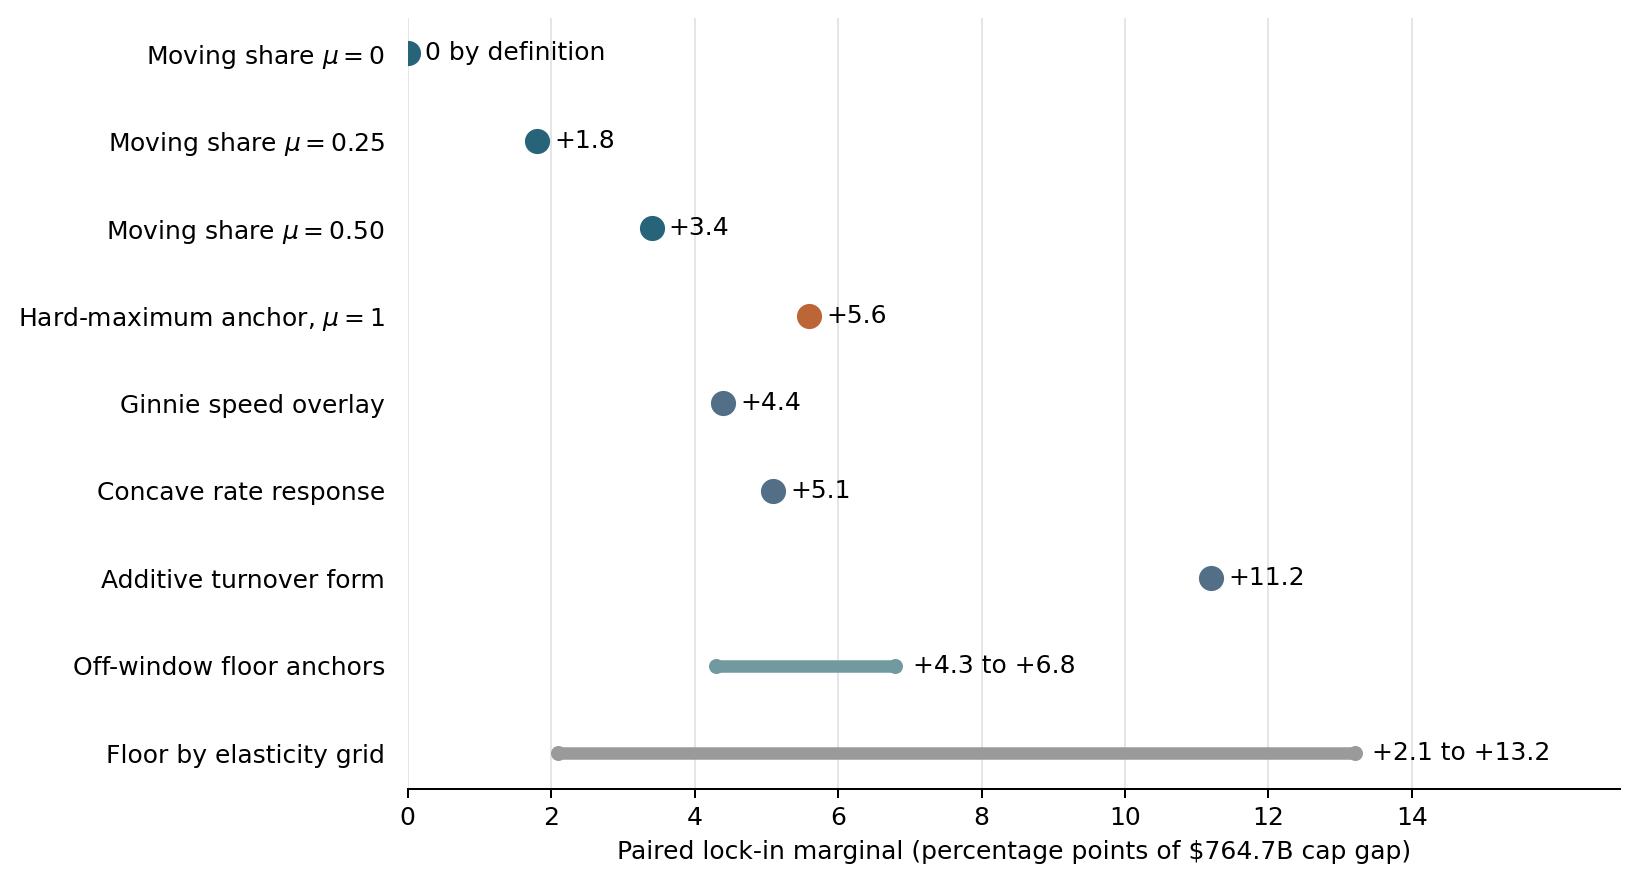
\includegraphics[width=0.95\textwidth]{fig13_specification_sensitivity}
\caption{Separate assumption comparisons from precise saved paired results. Each row names the changed input; all use the saved sample, 4.991\% annual floor, full moving share, maximum form, and 100 PSA except the named change. Values are points of the \$764.748253 billion gap. Rows are neither additive nor confidence intervals. The zero-share point is definitional. Sources and hashes are saved with the figure.}
\label{fig:band}
\end{figure}

\subsection{Stock-flow comparison}

The instrumented production calculation reproduces \$42.6083938811 billion within $1.2\times10^{-13}$ billion. Its response-off and response-on reported principal totals are \$692.582 and \$649.974 billion. Under the once-scaled closed-book convention they are \$679.776 and \$642.774 billion, giving \$37.0024 billion, or $+4.8385$ benchmark points. The change is $-\$5.6060$ billion, $-0.7331$ points, or $-13.16\%$ of the production marginal. The result therefore depends materially on the flow-reporting convention without implying that balances were previously reset each month.

Scheduled principal illustrates why common rules do not guarantee cancellation: it totals \$194.978 billion off and \$196.479 billion on in the closed book. Default-state transfers are approximately \$0.276 billion in each leg and are retained as claims, not treated as received principal. The production response-off report exceeds the phase-in cap in two months by \$0.0158 billion in total; cap enforcement reduces its paired runoff difference to \$42.5926 billion. Neither closed-book leg reaches a cap, so its principal and cap-allowed differences coincide. These are modeled implications, not estimates of the actual \$32.8 billion of phase-in purchases.

\subsection{Supported cells and the coupon bridge}

\begin{table}[H]
\centering\small
\caption{Three named populations and two reporting conventions. Dollar columns expand each pool to total initial holdings. The last column is closed-book marginal principal per \$100 initial active pool balance, not a measured supported-slice contribution.}
\label{tab:populationresults}
\begin{tabular}{@{}p{5.5cm}rrr@{}}\toprule
Sample & Reported (\$B) & Closed (\$B) & Per \$100\\\midrule
Saved production sample & 42.6084 & 37.0024 & 1.3658\\
Saved sample, joint cells & 36.5234 & 32.1965 & 1.1884\\
Fresh survivors, 80 bp & 42.1761 & 37.0584 & 1.3678\\
\bottomrule
\end{tabular}
\end{table}


The supported pool's initial active balance is approximately \$2{,}709.328 billion after the explicitly assumed whole-pool scale. Table~\ref{tab:populationresults} also expresses closed-book principal differences per \$100 of that initial active balance. This normalization states the conditional pool calculation without claiming that the 47.6\% book slice generated the displayed whole-pool dollars. A slice contribution would require a specified slice exposure and purchase path, which the current mapping does not provide.

All twelve cells remain supported with the same 75,000 fresh IDs at bridges of 60, 80, and 100 basis points, and initialized balance shares match within $10^{-8}$. The production-reported marginals are \$36.9512, \$42.1761, and \$45.3018 billion ($+4.8318/+5.5150/+5.9237$ points). The 80-bp result reproduces the saved fresh calculation. The bridge does not alter hazard note rates; it changes cell assignment and weights. The alternatives are diagnostic assumptions, not an empirically established plausible range. Appendix~\ref{app:population} gives support counts and weighting details.

\subsection{Frozen retrospective predictive check}\label{sec:validation}

Before scoring, the revision fixes the available panel, dates, exposure definition, state initialization, candidates, and subperiods. It uses January 2024--September 2025: 5,019 cohort-months in 239 supported vintage-coupon-credit-leverage cells over 21 months. These outcomes were previously examined in Path A and machine-learning diagnostics, so this is a frozen retrospective check, not an untouched holdout. The panel has no later October--November outcomes for this exercise and no loan IDs for an individual split.

Observed voluntary prepaid principal is the panel's prior-balance sum for voluntary payoff events. Opening exposure is reconstructed from the prior contiguous month's end exposure. Scheduled principal, default receipts, and curtailment are excluded on both sides because their separate observed components are unavailable. Predictions condition on realized opening exposure and rates. They use pre-evaluation age/covariate initialization and predicted-only burnout updates. The simple comparator is each cell's 2023 prepaid-principal-to-exposure rate; no evaluation outcome enters it. Appendix~\ref{app:validation} reports exclusions, cell ratios, and fixed half-year errors.

\begin{table}[H]
\centering\small
\caption{Legacy-input retrospective conditional prediction, January 2024--September 2025. Recorded prepaid principal is \$131.303 billion across 5,019 cohort-months. Dollars use preserved Freddie panel exposure. RMSE is exposure-weighted, in monthly probability percentage points.}
\label{tab:validation}
\begin{tabular}{@{}p{6cm}rrr@{}}\toprule
Candidate & Predicted (\$B) & P/O & RMSE\\\midrule
2023 cohort-speed baseline & 121.436 & 0.925 & 0.0868\\
Response off & 172.643 & 1.315 & 0.1570\\
Response on & 161.784 & 1.232 & 0.1339\\
\bottomrule
\end{tabular}
\end{table}


The response-on model improves on the response-off model, reducing exposure-weighted monthly-rate RMSE from 0.1570 to 0.1339 percentage points. It still performs worse than the 2023 comparator's 0.0868 points and predicts \$161.784 billion against \$131.303 billion observed. Its aggregate prediction/observation ratio is 1.232, versus 1.315 off and 0.925 for the comparator. Those are Freddie cohort dollars on observed exposure, not scaled SOMA dollars. The adverse result is retained without recalibration. It supports no claim that the imported elasticity, forward balance dynamics, or causal portfolio effect has been independently validated.

\subsection{Sampling uncertainty and other checks}

Sampling intervals condition on the model choices above. The loan-resampling procedure draws 130 vintage-by-coupon-by-FICO strata, with effective balance-weighted cluster count 25.8. At the 4.991\% floor its 200-replication percentile interval is $+4.631$ to $+6.924$ points; at the separate in-sample 4\% floor the interval is $+8.27$ to $+10.19$. These are distinct from the floor-read inference, which uses 31 cohort strata and only 5.87 effective clusters. The latter's restricted wild-cluster construction maps to $+1.9$ to $+9.1$ points under the stated maximum-form, central-response specification. Coverage simulations support the construction under their imposed cluster-shock design, not under arbitrary dependence or uncertain model form (Appendix~\ref{app:inference}).

A Fannie replication checks conventional-agency transport but uses the same imported elasticity and cannot independently validate it. Ginnie speed overlays, vintage checks, and the 15-year scheduled-principal extension have separate scope and proxy assumptions. An alternative household-choice model performs poorly on the aggregate benchmark; recalibration on real covariates substantially changes that comparison, so it does not establish a general superiority of one modeling approach. A fitted cohort hazard model also has unstable propagated uncertainty. The appendix retains these adverse checks.

No estimator explains the empirical month-to-month path reliably. The loan-level model's apparent aggregate relationship disappears after detrending, and incorrect seasonal rotations can perform similarly to the intended calendar. The calculation concerns cumulative principal differences, not the month in which that principal would otherwise have arrived.

\begin{figure}[H]
\centering
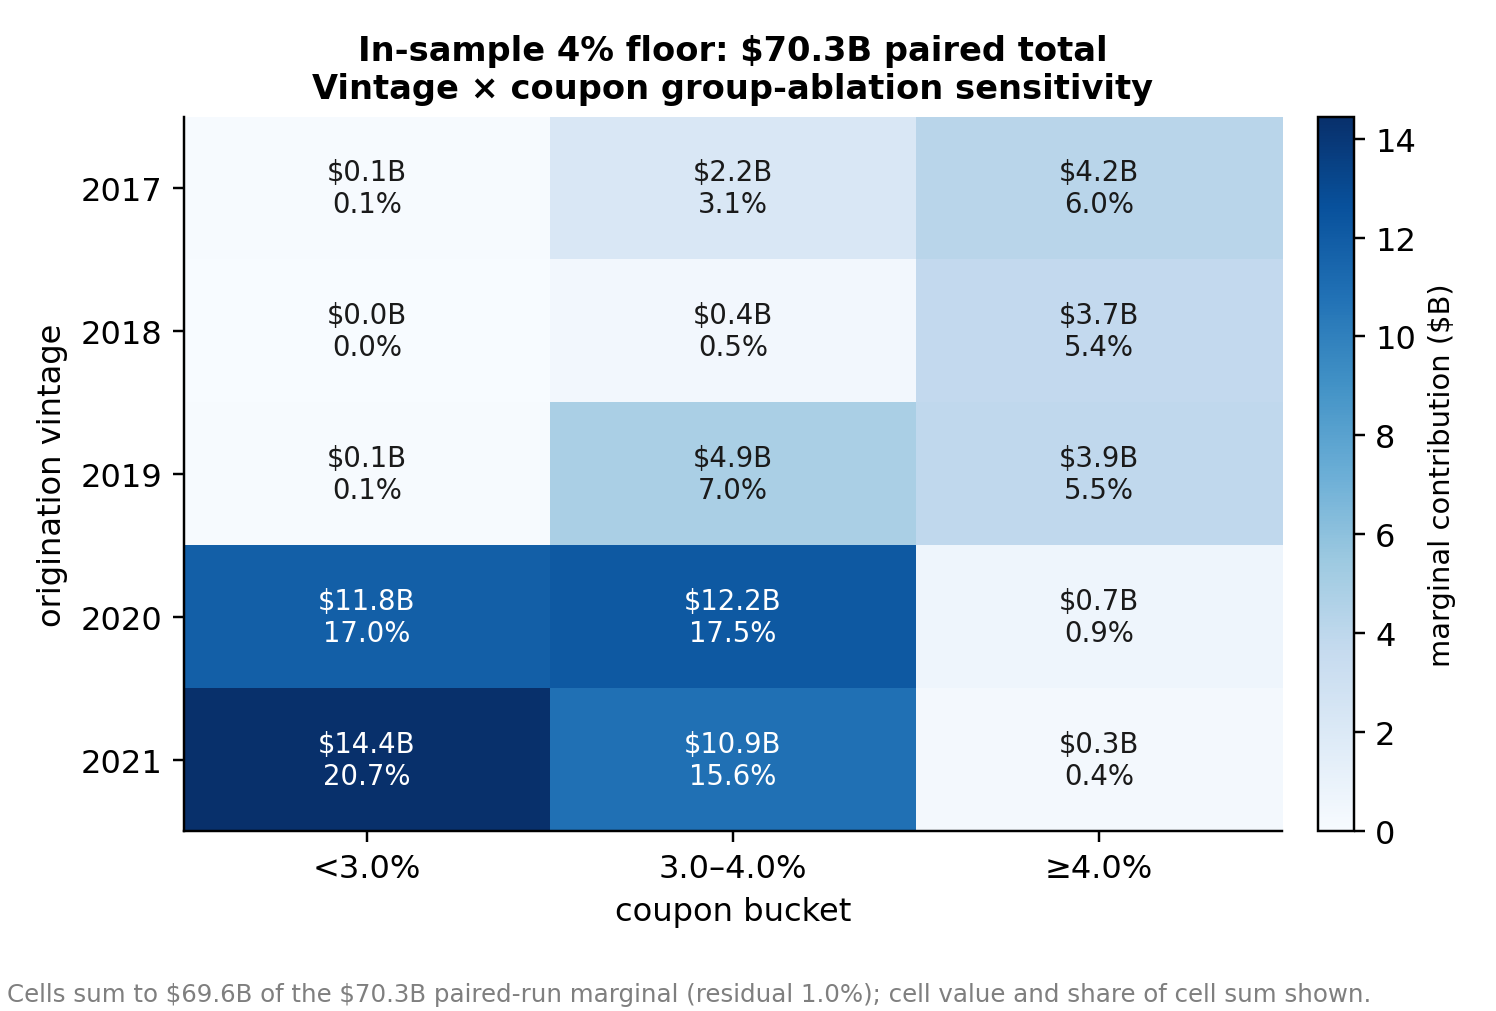
\includegraphics[width=0.77\textwidth]{fig11_marginal_decomposition}
\caption{Historical in-sample sensitivity: 4\% annual floor, 100 PSA, full moving share, saved sample, \$70.345 billion paired total. Group-ablation cells sum to \$69.620 billion; the \$0.725 billion residual is 1.03\% of the paired total. This figure does not allocate the \$42.608 billion off-window result. Values describe modeled coupon-vintage contributions, not differential causal effects.}
\label{fig:marginalcells}
\end{figure}

\section{Policy Implications}\label{sec:policy}

The cap is an operational limit and should be presented as such. The New York Fed already publishes balance-sheet projections; the proposal here is an incremental disclosure, not a claim that projections do not exist. A regularly updated side-by-side table would show the MBS cap, projected gross principal, expected reinvestment settlements, and projected net face decline, with the horizon and initial portfolio stated. Separate scenarios would change the interest-rate path and the prepayment assumptions. A reconciliation to subsequently realized cash flows and holdings would distinguish forecast error from settlement timing.

This is more informative than treating a conditional model-sensitivity band as a probabilistic forecast. The moving-share, PSA, and turnover-form comparisons have no assigned scenario probabilities. Publishing them would reveal why a cap can stay far above projected payments while reducing the risk that the gap is read as unanticipated policy failure. Household lock-in may remain important for mobility and welfare even when its conditional contribution to Federal Reserve runoff is much smaller than the full cap gap. This paper does not measure those welfare costs or feedback from mobility to prices and mortgage spreads.

Contract reform raises a separate question. Denmark's market-value repayment mechanism can reduce the penalty from extinguishing below-market debt \citep{campbell2013,berg2018,andersen2020}. A U.S. transplant's sign changes with assumed baseline mobility and with whether retired face or cash paid is counted. Appendix~\ref{app:alternatives} retains those signed comparisons and the source's working-paper status. The exercise does not price a transition in U.S. issuance, guarantees, servicing, or TBA liquidity and therefore does not justify a contract-policy recommendation from runoff dollars alone.

\section{Conclusion}\label{sec:conclusion}

The \$764.7 billion difference between announced MBS caps and realized net face decline is not a causal estimate of mortgage lock-in. The contemporaneous holdings projection anticipated most of that accounting gap under the two disclosed annual-allocation rules. A paired simulation can translate an imported household response into portfolio principal, but the translation depends on assumptions the aggregate data do not identify.

At the saved-sample maximum-form specification, assumed moving shares of 0, 25, 50, and 100\% give $0$, $+1.8$, $+3.4$, and $+5.6$ points, respectively. The \$42.6 billion full-share result is not an empirically preferred estimate. At that floor, the 75--150 PSA sweep spans $+0.9$ to $+15.6$ points; the survival-combination form gives $+11.2$ at 100 PSA; and once-scaled closed-book accounting gives \$37.0 billion for the original sample. The fresh supported-cell and bridge comparisons are conditional whole-pool calculations, not actual contributions from the 47.6\% supported slice.

The retrospective check improves on response off but loses to a simple cohort-speed baseline. Sale-reason data, broader collateral coverage, and untouched loan-level evaluation remain needed to strengthen the empirical interpretation. The current contribution is a transparent accounting decomposition with material assumptions and adverse evidence visible beside its results. The operational recommendation is to publish updated cap and cash-flow scenarios together, with separate rate and prepayment assumptions and an explicit bridge from gross principal to net holdings.

\clearpage
\singlespacing
\bibliographystyle{plainnat}
\bibliography{references}
\clearpage
\appendix
\noindent\textbf{Online Appendix.} Economics-review revision, October 7, 2026. The dated replication archive preserves the reviewed manuscript, superseded specification history, original results, and prior adjudication notes. This appendix contains the current derivations, material sensitivities, and adverse checks. Its tables use precise saved artifacts; rounding is for display only.

\section{Model Equations and Monthly Accounting}\label{app:model}

Equation~\eqref{eq:beta1} converts a proportional change in a quarterly probability into a monthly log-hazard coefficient. It does not divide the quarterly percentage response by three. At $P=0.06$, baseline monthly probability is $1-0.94^{1/3}=0.020414$; the shocked quarterly probability is $0.0561$. Their monthly probability ratio gives $b=-0.0685705$. The exponent's sign in equation~\eqref{eq:pathB} is negative for a positive market-minus-note gap. At 380 bp it is $-0.260568$, yielding a 0.771 hazard multiplier before the floor and competing-risk normalization. The reference probability and extrapolation to large gaps remain assumptions.

The production default trigger is
\begin{equation}
h^D_{it}=0.0003\exp\{2\max(0,r_t-c_i)-0.20z_i^{\mathrm{FICO}}+0.25z_i^{\mathrm{LTV}}\},
\label{eq:default}
\end{equation}
clipped to $[0,1]$. Here rate stress is in decimals, unlike the percentage-point gap in the prepayment exponent. If $h^P+h^D>1$, both are divided by their sum. The fractional voluntary payment is then $B_{it}^{open}h^P_{it}$. A uniform default trigger first moves a current loan to 30-day delinquency or an already delinquent loan to default. The Markov transition matrix advances delinquent states. Default/liquidated states are inactive; the current engine supplies no recovery cash from those balances. It does not model a foreclosure-recovery lag with measured receipts.

\begin{table}[!htbp]
\centering\small
\caption{Code-to-equation and timing map for the current calculation.}
\label{tab:modelmap}
\begin{tabular}{@{}>{\raggedright\arraybackslash}p{3.5cm}>{\raggedright\arraybackslash}p{5.2cm}>{\raggedright\arraybackslash}p{5.7cm}@{}}\toprule
Object & Equation or definition & Implementation location\\\midrule
Imported response & Equation~\eqref{eq:beta1}, negative code coefficient & \path{literature_hazard.rothstein_beta1}\\
PSA baseline & Equation~\eqref{eq:psa}; monthly probability & \path{literature_hazard.h0_psa}\\
Voluntary hazard & Equation~\eqref{eq:pathB}, sample covariates and stratum burnout & \path{literature_hazard.prepay_hazard}\\
Floor combination & Equations~\eqref{eq:maxfloor}--\eqref{eq:addfloor}; annual floor converted first & Same prepayment function\\
Default & Equation~\eqref{eq:default}; monthly trigger then state transitions & \path{competing_risks.monthly_step}\\
Burnout & Cumulative prepaid/original stratum principal; cap at one & Updated after default triggers, before Markov transitions\\
Amortization & Note-rate annuity principal on post-prepayment active balance & \path{macro.scheduled_amortization_smm}\\
Dollar reporting & Equation~\eqref{eq:reporting}; closing active denominator & \path{microsim_engine._simulate_regime}\\\bottomrule
\end{tabular}
\end{table}

Scheduled principal is computed after fractional prepayment and delinquency transitions, using the loan's note rate, 360-month amortization term, and elapsed age. The engine's diagnostic exposure field adds prepayment back to remaining balances but does not add scheduled principal back; it is not an exact beginning-of-month denominator. The new stock-flow comparison instead records opening and closing balances explicitly. The retrospective check constructs its own contiguous lagged exposure, independently of that diagnostic field.

Write $A_t$ for active principal, $I_t$ inactive principal claims, $V_t$ voluntary cash principal, $S_t$ scheduled principal, and $D_t$ transfers to inactive claims. In the closed opening book,
\begin{align}
A_{t+1}&=A_t-V_t-S_t-D_t,\label{eq:activebalance}\\
I_{t+1}&=I_t+D_t,\qquad
(A+I)_{t+1}=(A+I)_t-V_t-S_t.\label{eq:totalbalance}
\end{align}
There are no additions, curtailment receipts, or default recovery receipts in this scoped comparison. An absorbing-state transfer is not counted a second time as cash. The maximum absolute monthly active-identity error is below $10^{-12}$ billion in both original-sample legs. Initial total principal is \$2{,}709.328 billion; initial active principal is \$2{,}709.266764 billion, with the difference already inactive. These are explicit scale assumptions, not the supported slice's observed principal.

The production reporting denominator is closing active exposure. Its use is reproduced, not silently repaired. The once-scaled comparison removes this reporting operation and therefore measures a different dollar object. It omits unsettled purchases and future reinvestment pools because the present loan data do not identify them. A comparable full-book counterfactual would need settlement-level purchases, reinvestment allocation, collateral composition, and default remittances. Common historical shared-layer adjustments cancel only because the same external dollars are imposed on both legs; equation~\eqref{eq:totalbalance} does not imply cancellation of scheduled principal generated by changing balances.

\section{Retrospective Cohort Prediction}\label{app:validation}

The available cohort panel contains 22,709 rows from January 2017 through September 2025. Earlier analyses already used the post-2023 period for model diagnostics. The new exercise is frozen before scoring in the dated validation specification, with pre-evaluation comparator training during calendar 2023 and evaluation in 2024--September 2025. No claim of statistical independence follows from that retrospective freeze.

The risk set is a cohort, not an individual loan: vintage, 50-bp note-coupon, FICO bucket, and LTV bucket. The panel lacks loan IDs and separate default, scheduled, and curtailment amounts. Voluntary payoff includes the data's ``prepaid or matured'' category, not just property sales. Observed events use the preceding balance of a voluntary-payoff loan. Opening exposure is the prior contiguous cohort end balance; observations with missing/noncontiguous exposure or events above exposure are excluded rather than clipped into a valid probability. Across the full input, 298 rows lack a usable contiguous lag and one has an invalid numerator. An additional 1,058 otherwise usable evaluation rows lack the frozen training, December-2023, or saved-sample covariate support. The retained balanced evaluation contains 239 cohorts and 5,019 monthly rows. All 6,077 evaluation rows have usable lagged exposure and numerators before the support restriction. The retained rows cover 99.9946\% of that exposure and 99.9935\% of its observed principal; the saved artifact records both denominators.

The comparator fixes each retained cohort's 2023 total prepaid principal divided by its total opening exposure. Model candidates retain 100 PSA, 4.991\% floor, maximum form, and the original coefficients. Cell credit/leverage inputs are averages of standardized saved-sample characteristics; age starts at December 2023 and advances mechanically. Burnout starts at its December-2023 value and subsequently increases from predicted prepayment, never evaluation outcomes. This aggregation and burnout projection approximate the loan-level model. Realized opening exposures and mortgage rates are conditioning information, so this is not a free-running balance or ex-ante rate forecast.

For cohort-months $j$, observed principal $Y_j$, opening exposure $E_j$, and predicted monthly probability $\widehat h_j$, the reported error is
\begin{equation}
\mathrm{RMSE}_w=100\sqrt{\frac{\sum_j E_j(\widehat h_j-Y_j/E_j)^2}{\sum_j E_j}},\qquad
\mathrm{P/O}=\frac{\sum_j E_j\widehat h_j}{\sum_jY_j}.
\label{eq:validation}
\end{equation}
RMSE is in monthly probability percentage points, not annual CPR points. Cumulative principal is on the observed Freddie exposure base. All three candidates use the same retained observations. Table~\ref{tab:validperiods} shows fixed subperiods; Table~\ref{tab:validcells} shows coupon-vintage totals so aggregate error cannot hide offsetting cells. Zero-observed cells would have an undefined ratio rather than a manufactured zero.

\begin{table}[H]
\centering\small
\caption{Fixed evaluation subperiods: prediction/observation ratio and monthly weighted RMSE. The final half-year ends September 2025.}
\label{tab:validperiods}
\begin{tabular}{@{}lrrrr@{}}\toprule
Period & Observed (\$B) & Baseline P/O; RMSE & Off P/O; RMSE & On P/O; RMSE\\\midrule
2024H1 & 36.353 & 1.005 / 0.0862 & 1.436 / 0.1825 & 1.338 / 0.1551\\
2024H2 & 38.864 & 0.901 / 0.0728 & 1.282 / 0.1435 & 1.202 / 0.1215\\
2025H1 & 35.404 & 0.950 / 0.0909 & 1.346 / 0.1620 & 1.265 / 0.1391\\
2025H2 & 20.683 & 0.786 / 0.1053 & 1.110 / 0.1030 & 1.048 / 0.0899\\
\bottomrule
\end{tabular}
\end{table}

{\small
\begin{longtable}{@{}lrrrrr@{}}
\caption{Coupon-vintage validation totals. Ratios retain all candidates on the same cells; dollars are observed prepaid principal.}\label{tab:validcells}\\
\toprule
Vintage; note coupon & Rows & Observed (\$B) & Baseline P/O & Off P/O & On P/O\\\midrule
\endfirsthead
\toprule
Vintage; note coupon & Rows & Observed (\$B) & Baseline P/O & Off P/O & On P/O\\\midrule
\endhead
2017; 2\% & 21 & $<0.001$ & 0.000 & 11.401 & 11.401\\
2017; 2.5\% & 42 & 0.001 & 0.604 & 0.910 & 0.894\\
2017; 3\% & 126 & 0.200 & 1.018 & 0.951 & 0.948\\
2017; 3.5\% & 126 & 0.404 & 1.020 & 0.930 & 0.929\\
2017; 4\% & 126 & 2.951 & 1.060 & 0.965 & 0.964\\
2017; 4.5\% & 126 & 1.361 & 1.079 & 0.897 & 0.893\\
2017; 5\% & 126 & 0.697 & 1.080 & 0.799 & 0.790\\
2017; 5.5\% & 126 & 0.030 & 1.026 & 0.705 & 0.692\\
2017; 6\% & 84 & 0.004 & 0.894 & 0.615 & 0.592\\
2018; 2.5\% & 21 & 0.000 & -- & -- & --\\
2018; 3\% & 84 & 0.015 & 1.055 & 0.910 & 0.909\\
2018; 3.5\% & 126 & 0.058 & 0.972 & 0.905 & 0.904\\
2018; 4\% & 126 & 0.716 & 1.028 & 0.874 & 0.873\\
2018; 4.5\% & 126 & 1.226 & 1.086 & 0.854 & 0.853\\
2018; 5\% & 126 & 2.020 & 1.128 & 0.824 & 0.820\\
2018; 5.5\% & 126 & 0.426 & 1.086 & 0.712 & 0.705\\
2018; 6\% & 126 & 0.178 & 1.103 & 0.649 & 0.643\\
2018; 6.5\% & 84 & 0.005 & 0.917 & 0.621 & 0.621\\
2019; 2\% & 21 & $<0.001$ & 0.000 & 19.473 & 19.473\\
2019; 2.5\% & 63 & 0.007 & 0.848 & 1.360 & 1.311\\
2019; 3\% & 126 & 0.499 & 0.953 & 1.073 & 1.072\\
2019; 3.5\% & 126 & 1.714 & 0.974 & 1.081 & 1.080\\
2019; 4\% & 126 & 5.021 & 1.037 & 0.953 & 0.952\\
2019; 4.5\% & 126 & 1.680 & 1.076 & 0.832 & 0.829\\
2019; 5\% & 126 & 1.150 & 1.097 & 0.773 & 0.768\\
2019; 5.5\% & 126 & 0.283 & 1.025 & 0.645 & 0.640\\
2019; 6\% & 126 & 0.122 & 1.120 & 0.616 & 0.612\\
2019; 6.5\% & 105 & 0.007 & 0.823 & 0.582 & 0.579\\
2019; 7\% & 63 & 0.000 & -- & -- & --\\
2020; 2\% & 126 & 0.888 & 0.896 & 1.723 & 1.667\\
2020; 2.5\% & 126 & 6.478 & 0.902 & 1.675 & 1.607\\
2020; 3\% & 126 & 26.963 & 0.939 & 1.390 & 1.328\\
2020; 3.5\% & 126 & 8.426 & 0.962 & 1.089 & 1.068\\
2020; 4\% & 126 & 2.838 & 1.013 & 0.941 & 0.936\\
2020; 4.5\% & 126 & 0.346 & 1.003 & 0.814 & 0.810\\
2020; 5\% & 126 & 0.264 & 1.028 & 0.691 & 0.684\\
2020; 5.5\% & 126 & 0.041 & 1.129 & 0.559 & 0.558\\
2020; 6\% & 105 & 0.014 & 0.837 & 0.494 & 0.493\\
2021; 2\% & 126 & 2.795 & 0.812 & 1.641 & 1.566\\
2021; 2.5\% & 126 & 7.792 & 0.860 & 1.648 & 1.551\\
2021; 3\% & 126 & 41.126 & 0.864 & 1.443 & 1.308\\
2021; 3.5\% & 126 & 9.853 & 0.908 & 1.232 & 1.070\\
2021; 4\% & 126 & 2.208 & 0.898 & 1.060 & 0.922\\
2021; 4.5\% & 126 & 0.368 & 0.943 & 0.847 & 0.758\\
2021; 5\% & 105 & 0.127 & 0.921 & 0.759 & 0.697\\
2021; 5.5\% & 63 & 0.003 & 0.821 & 0.558 & 0.520\\
\bottomrule
\end{longtable}
}


The response-on candidate performs worse than the simple comparator in aggregate; it is not selected or recalibrated after seeing this result. A future prospective check would freeze eligible loan IDs, opening balances, subsequent observation dates, censoring/default treatment, all coefficients, and comparator rules before access to genuinely unseen performance. It would separately score voluntary, scheduled, default, and total principal using observed event histories and beginning balances. That evaluation has not occurred here, and passing code or document checks cannot substitute for it.

\section{Population, Weighting, and Bridge Support}\label{app:population}

The fresh draw uses the twenty 2017Q1--2021Q4 compact survivor snapshots and seed 42. All 75,000 IDs are unique. It is sampled from Freddie May-2022 30-year survivors with positive principal, then matched to twelve listed June-29-2022 UMBS coupon-vintage cells. Their 47.5876\% share is of total SOMA MBS face, while within-target weights sum to one. The UMBS grid cannot determine the Freddie/Fannie collateral mix, and omitted cells below the listing threshold remain unrepresented. All recorded sample/output/code and snapshot hashes match the saved audit.

For bridge $b$ basis points, the bucket is the nearest 50-bp increment to $c_i-b/10{,}000$. Original note coupons remain unchanged in hazards and amortization. Within cell $k$, balance weights multiply original balance by the target share divided by its original cell balance share. Both response legs use precisely the same resulting weights and ID order. A missing positive-target cell stops that bridge comparison and reports its missing target share; there is no silent renormalization. No such failure occurs for the fixed-ID 60/80/100-bp diagnostics. The fixed 75,000 candidate IDs have 69,613, 75,000, and 74,701 positive-weight loans at the three bridges; candidates outside the twelve targets receive zero weight. The smallest target cells have 42, 204, and 78 loans respectively; that thin support is a reason not to read the three points as an empirically calibrated interval.

\begin{table}[H]
\centering\small
\caption{Fixed-ID bridge support. Target shares condition on the twelve listed cells; their total face share is 47.5876\%. All targets match within $5.6\times10^{-17}$ at initialization.}
\label{tab:support}
\begin{tabular}{@{}lrrrr@{}}\toprule
Pass-through; vintage & Target & 60 bp loans & 80 bp loans & 100 bp loans\\\midrule
2\%; 2021 & 40.462\% & 12204 & 30347 & 36031\\
2.5\%; 2021 & 17.433\% & 29589 & 13074 & 4668\\
2.5\%; 2020 & 14.074\% & 12023 & 10555 & 6260\\
2\%; 2020 & 12.213\% & 3517 & 9160 & 13645\\
1.5\%; 2021 & 4.182\% & 202 & 3137 & 5657\\
3\%; 2017--19 & 3.388\% & 1151 & 2541 & 2521\\
3\%; 2020 & 2.654\% & 6228 & 1991 & 754\\
3.5\%; 2017--19 & 1.943\% & 2507 & 1458 & 1094\\
4\%; 2017--19 & 1.614\% & 1430 & 1210 & 1003\\
1.5\%; 2020 & 1.135\% & 42 & 851 & 1857\\
2.5\%; 2017--19 & 0.629\% & 56 & 472 & 1133\\
4.5\%; 2017--19 & 0.272\% & 664 & 204 & 78\\
\bottomrule
\end{tabular}
\end{table}


The saved-sample joint run is \$36.5234 billion under production reporting, versus \$42.6084 billion for the saved unweighted specification. The fresh 80-bp joint run is \$42.1761 billion. Changing the frame as well as the draw prevents a sampling-only attribution of those differences. Whole-pool scaling is a separate assumption from within-support composition. Multiplying these dollars by 47.6\% without a defined slice exposure path would not produce an observed supported-slice contribution.

\section{Conditional Inference and Calibration}\label{app:inference}

The 130 loan-draw strata are vintage year $\times$ 50-bp coupon $\times$ FICO bucket. A cluster replication samples strata with replacement and takes all their loans, so total loan count varies. Two hundred paired replications hold the engine seed at 42. Effective cluster count is $1/\sum_k w_k^2=25.78$, using initial balance shares; the largest share is 9.77\%. The 4.991\%-floor marginal has median $+5.641$ points and percentile endpoints $+4.631,+6.924$ (\$35.415--\$52.954 billion). These intervals refer to the saved sample, full moving share, 100 PSA, maximum form, and production reporting.

The floor read instead selects 2018 cohort-months with age at least twelve and note-minus-market gap at most $-0.25$ percentage points. Its clusters are vintage $\times$ coupon $\times$ FICO $\times$ LTV, preserving repeated-month dependence within 31 strata. Exposure concentration reduces its effective count to 5.87; maximum leverage is 0.332. The restricted Webb wild-cluster test inversion uses 9,999 draws and 401 candidate floor values, with the floor mapped through the fixed marginal-response grid. Its reported $+1.9$ to $+9.1$ point interval conditions on the central imported response and maximum form. It does not cover uncertainty about moving share, PSA, coefficient transport, portfolio mapping, or reporting convention.

The coverage exercise imposed the observed cluster-weight pattern with Gaussian or $t_5$ cluster shocks in 5,000 outer simulations and 999 inner draws. Restricted Webb coverage was 94.34\% and 95.08\%, respectively. This tests a stated synthetic error design; it does not establish coverage under arbitrary time shocks, selection into discount cohorts, or uncertain hazard structure. Month and two-way-cluster sensitivity remains in the replication record. No bootstrap was rerun to correct the cluster descriptions.

\begin{table}[H]
\centering\small
\caption{Separate uncertainty objects; each interval retains its own specification.}
\label{tab:inference}
\begin{tabular}{@{}>{\raggedright\arraybackslash}p{4.5cm}>{\raggedright\arraybackslash}p{3.1cm}>{\raggedright\arraybackslash}p{6.8cm}@{}}\toprule
Object & Points of cap gap & Conditioning and interpretation\\\midrule
Loan-stratum percentile, 4.991\% floor & $+4.631$ to $+6.924$ & 130 nominal / 25.78 effective clusters; sample variation only.\\
Loan-stratum percentile, 4\% floor & $+8.27$ to $+10.19$ & Historical in-sample floor; different center.\\
Floor-read restricted wild interval & $+1.9$ to $+9.1$ & 31 nominal / 5.87 effective clusters; fixed response/form.\\
Floor--elasticity grid & $+2.1$ to $+13.2$ & Assumption sweep, not a sampling interval.\\
PSA 75--150 at 4.991\% floor & $+0.856$ to $+15.626$ & Fixed full share and maximum form; not a confidence band.\\\bottomrule
\end{tabular}
\end{table}

Baseline transport remains uncertain. Calendar standardization moves the named marginal to about $+4.7$ points; housing-activity rescaling moves it to about $+10.7$. Alternative covariate and burnout choices remain saved with their exact specifications. None transforms observed 2018 discount turnover into an identified, purely non-rate component. The in-sample 4\% floor's group-ablation figure remains explicitly labeled: \$70.345 billion paired total, \$69.620 billion cell sum, \$0.725 billion residual from interactions. Its shares are not rescaled to the off-window specification.

\section{Benchmarks, Settlement Diagnostics, and Loan Life}\label{app:benchmark}

The original report/workbook source trail is independent of the later September-2022 policy explainer. The five workbook year-end MBS levels telescope to a \$765.8 billion 2021--2025 decline. Uniform calendar allocation leaves \$740.583 billion in June-2022--November-2025. The settlement-aware adjustment first adds the \$92.322 billion early-year holdings-rise proxy to 2022's net decline, assigns the resulting \$108.222 billion to June--December, and gives \$839.530 billion in the full window. It is a disclosed allocation using realized early-year information, not an untouched forecast.

\begin{table}[H]
\centering\small
\caption{Within-year allocation stress cases from the saved projection comparison. All keep realized net face decline at \$652.752 billion.}
\label{tab:allocationstress}
\begin{tabular}{@{}p{7cm}rrr@{}}\toprule
Allocation change from uniform & Projected decline & Gap & Anticipated share\\\midrule
2022 linear back-loaded annual net & 744.151 & 91.399 & 88.05\%\\
All 2025 decline in January--November & 759.175 & 106.423 & 86.08\%\\
All 2025 decline in December & 536.075 & $-116.677$ & 115.26\%\\\bottomrule
\end{tabular}
\end{table}

The all-December case is an implausible boundary stress, not a likely scenario. Its negative expectations-relative gap is a surplus under that allocation. It shows why there is no unique ratio of the model marginal to a projection-relative denominator.

A separate timing diagnostic convolves the cap with the $(0.1,0.6,0.3)$ monthly lag kernel while keeping realized holdings changes unchanged. The benchmark becomes \$722.748 billion because exactly \$42 billion of cap mass is pushed beyond November 2025. Faster/slower kernels give \$736.748 and \$712.248 billion. These are window-edge effects of convolving a schedule, not a reconstruction of actual mortgage remittances. The named calendar-convention gap remains \$764.748253 billion. Phase-in purchases and settlement timing make any gross-principal interpretation particularly inappropriate at the opening boundary.

Weighted-average-life calculations are scenario illustrations with explicit coupon and CPR bases. Table~\ref{tab:wal} restores an actual loan-life reference; it no longer points to an unrelated validation table. The empirical note-rate row uses a 5.79\% CPR back-out and the 80-bp coupon conversion in its amortization basis. The turnover-floor row is a separate constant-CPR illustration, not a fitted lifetime forecast. They cannot be differenced against a no-shock row on another convention to infer an identified duration effect.

\begin{table}[H]
\centering\small
\caption{Approximate weighted-average life (years), with scenario and basis stated.}
\label{tab:wal}
\begin{tabular}{@{}lrrr@{}}\toprule
Scenario & Annual CPR & June 2022 & November 2025\\\midrule
Empirical back-out, note-rate basis & 5.79\% & 8.9 & 8.1\\
Empirical back-out, hazard basis & 5.52\% & 9.1 & 8.3\\
Off-window turnover-floor illustration & 4.99\% & 9.5 & 8.6\\\bottomrule
\end{tabular}
\end{table}

\section{Adverse Checks and Institutional Extensions}\label{app:alternatives}

The fitted cohort hazard approach (Path A) estimates associations in the Freddie panel. Its prior-specification coefficient bootstrap is skewed and its full forward simulations have unstable tails; its newer calendar-seasonal specification does not carry a reliable recomputed inferential object. It is not independent corroboration of the imported response. The aggregate level can also be reproduced using synthetic populations, indicating that calibration and survival mechanics can generate a close level match without identifying a causal effect.

The household-choice model's original aggregate recovery is about 13.6\% across simulation seeds, but recalibrating on real loan covariates raises its mean to 60.2\% and book-composition adjustment changes it further. The original contrast therefore does not isolate the modeling paradigm. These adverse results remain available in the archived derivations and frozen artifacts; their removal from the main narrative does not turn them into successful validation.

Fannie replication yields an in-sample marginal near $+8.68$ points versus Freddie's $+9.20$ at the 4\% floor. The common imported elasticity means this checks conventional-agency transfer of the calculation. A Ginnie speed overlay composed with the off-window floor gives approximately $+4.4$ points, with no directly estimated Ginnie elasticity or assumption take-up. The excluded-vintage observed-speed proxy gives an approximately \$11.7 billion level bound, conditional on Fannie segment speeds representing the book; it is not a direct estimate of the excluded loans' marginal. Fifteen-year collateral enters portfolio amortization without a separately estimated behavioral response. Each extension addresses a different dimension of coverage.

The Danish market-value repayment extension imports a separate working-paper calibration \citep{berger2026}. At the in-sample 4\% floor, a rule-only transplant retaining the U.S. zero-gap moving intercept gives $+\$61.2$ billion in retired face. Importing the Danish baseline mobility instead gives $-\$99.9$ billion, and the re-derived cash-incidence convention gives $-\$51.0$ billion. These signed comparisons use different anchors and cash/face objects. They are neither predictions for the U.S. book nor comparable estimates at the off-window \$42.6 billion specification. The exercise does not estimate the cost of changing U.S. issuance, guarantee-fee allocation, servicing contracts, or TBA liquidity. The July-2026 source is an unrefereed working paper, and its changing refinancing estimates are retained as a limitation.

\section{Replication Record}\label{app:replication}

Editable sources, numerical artifacts, code, specifications, input hashes, and a twelve-issue disposition report accompany this local edition. The reviewed 83-page combined PDF is preserved byte-for-byte under the dated baseline directory. The original main text, long abstract, and extensive online appendix are preserved under \texttt{reviewed\_archive}; superseded results and internal adjudications remain research history, not current conclusions. Current references attach to actual equations and exhibits, with a semantic audit of object types and selected destinations.

Freddie/Fannie raw data and loan-grain or potentially identifying compact panels are not redistributed in the source package. Reproduction of loan-based calculations requires the user's existing licensed local files. The new runs read compact saved inputs and a frozen public-macro extract, avoiding bulk raw downloads. Software and rendering checks establish reproducibility and document integrity within that environment; they do not establish causal identification, independent predictive success, or full-SOMA representativeness.

\end{document}
